\chapter{Shift Invariance of the $\DTCWT$}
\begin{figure}
  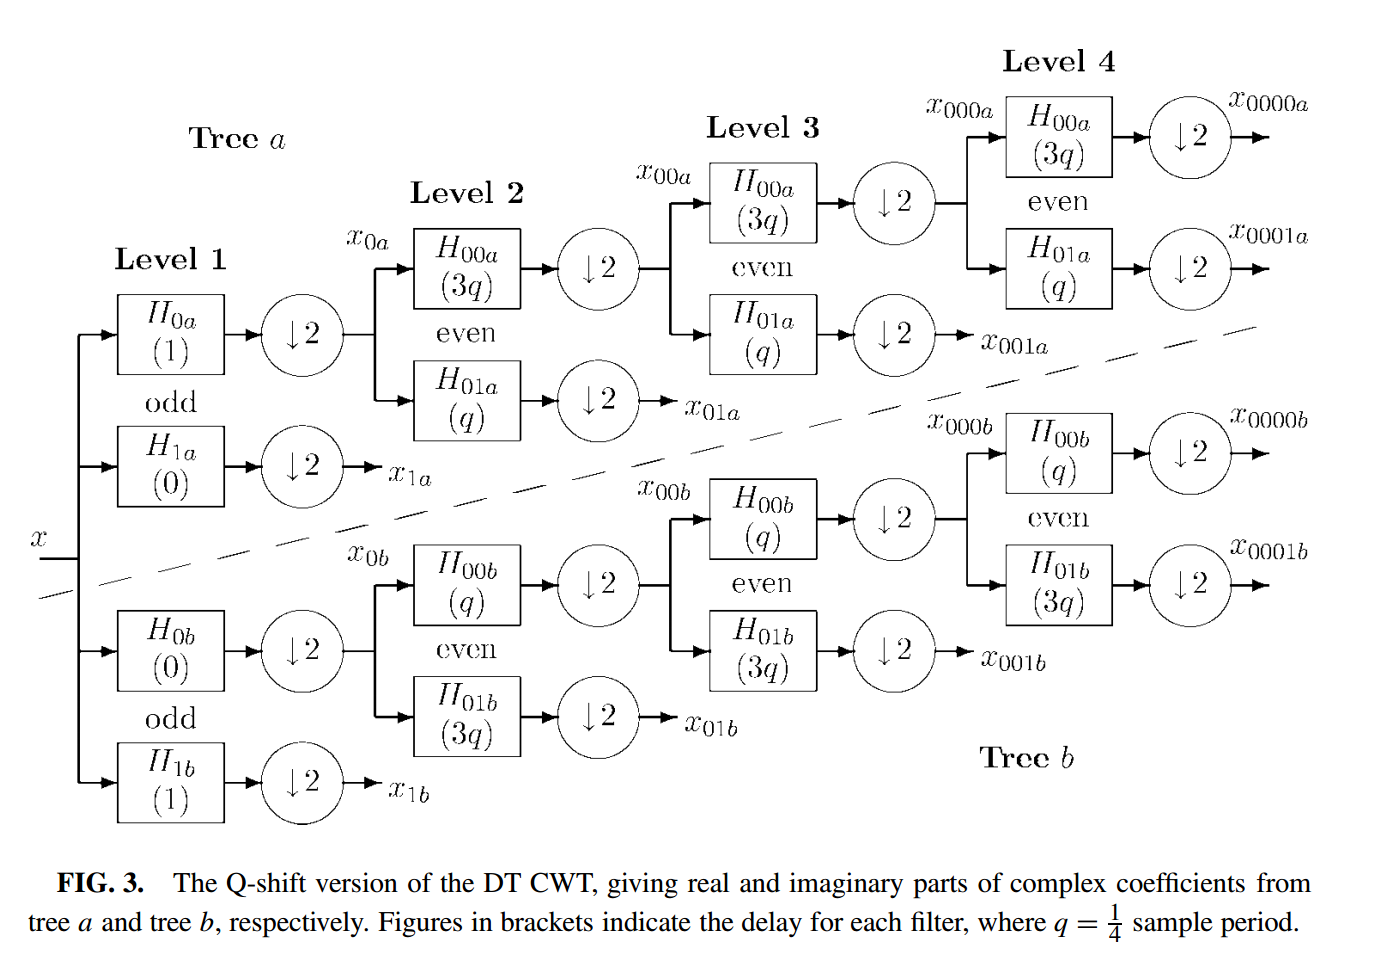
\includegraphics[width=\textwidth]{\imgpath/dtcwt.png}
  \mycaption{Full 1-D $\DTCWT$}{}
\end{figure}
\begin{figure}
  \centering
  \begin{tikzpicture}
    \matrix (m1) [minimum height=4mm, column sep=6mm, align=center]
	{
	%--------------------------------------------------------------------
		\node[coordinate]                  (m00) {};    &
		\node[coordinate]                  (m01) {};          &
		\node[dspsquare]                   (m02) {$A(z)$};          &
		\node[circle,draw,inner sep=1pt]   (m03) {\downsamplertext{M}}; &
		\node[dspnodeopen,dsp/label=above] (m04) {$X_a(z)$};          &
		\node[circle,draw,inner sep=1pt]   (m07) {\upsamplertext{M}}; &
		\node[dspsquare]                   (m08) {$C(z)$};          &
		\node[coordinate]                  (m09) {};          &
		\node[coordinate]                  (m0X) {};          \\
		%--------------------------------------------------------------------
		\node[dspnodefull]                 (m10) {};          &
		\node[coordinate]                  (m11) {};          &
		\node[coordinate]                  (m12) {};    &
		\node[coordinate]                  (m13) {};          &
		\node[coordinate]                  (m14) {};    &
		\node[coordinate]                  (m17) {};          &
		\node[coordinate]                  (m18) {};    &
		\node[dspadder]                    (m19) {};          &
		\node[]     (m1X) {};          \\
		%--------------------------------------------------------------------
		\node[coordinate]                  (m20) {};    &
		\node[coordinate]                  (m21) {};          &
		\node[dspsquare]                   (m22) {$B(z)$};          &
		\node[circle,draw,inner sep=1pt]   (m23) {\downsamplertext{M}}; &
		\node[dspnodeopen,dsp/label=below] (m24) {$X_b(z)$};          &
		\node[circle,draw,inner sep=1pt]   (m27) {\upsamplertext{M}}; &
		\node[dspsquare]                   (m28) {$D(z)$};          &
		\node[coordinate]                  (m29) {};          &
		\node[coordinate]                  (m2X) {};          \\
		%--------------------------------------------------------------------
	};
	\draw[dspline] (m10) -- (m11);
	\draw[dspline] (m11) -- (m01);
	\draw[dspline] (m11) -- (m21);
	\foreach \i in {0,2} {
    	\draw[dspconn] (m\i1) -- (m\i2);
    	\draw[dspconn] (m\i2) -- (m\i3);
    	\draw[dspline] (m\i3) -- (m\i4);
    	\draw[dspconn] (m\i4) -- (m\i7);
    	\draw[dspconn] (m\i7) -- (m\i8);
    	\draw[dspline] (m\i8) -- (m\i9);
	}
  \node[left=0pt of m10] (left) {$X(z)$};
  \node[below=9pt of m24] (bottom) {};
  \draw[dspconn] (m09) -- node[right, yshift=5pt] {$Y_a(z)$} (m19);
  \draw[dspconn] (m29) -- node[right, yshift=-5pt] {$Y_b(z)$} (m19);
  \draw[dspconn] (m19) -- node[right, xshift=5pt] {$Y(z)$} (m1X);
	
\end{tikzpicture}

  \mycaption{Block Diagram of 1-D $\DTCWT$}{Note the top and bottom paths are
  through the wavelet or scaling functions from just level m ($M=2^m$). Figure
  based on Figure~4 in \cite{kingsbury_complex_2001}.}
  \label{fig:ch2:dtcwt_two_tree}
\end{figure}
Firstly, let us look at what would happen if we retained only one of the subbands.
Note that we have to keep the same band from each tree. For any pair of
coefficients on the tree, this would look like \autoref{fig:ch2:dtcwt_two_tree}.
E.g.\ if we kept $x_{001a}$ and $x_{001b}$ then $M=8$ and $A(z) =
H_{0a}(z)H_{00a}(z^2)H_{001a}(z^4)$ is the transfer fucntion from $x$ to
$x_{001a}$. The transfer functions for $B(z)$, $C(z)$ and $D(z)$ are obtained
similarly. It is well known that:
\begin{align}
  U(z) \downarrow M &\rightarrow  U(z^M) \\
  U(z) \uparrow M &\rightarrow  \frac{1}{M}\sum_{k=0}^{M-1}U(W^kz^{1/M})
\end{align}
Where $W=e^{j2\pi/M}$. So downsampling followed by upsampling becomes:
\begin{equation}
U(z) \downarrow M \uparrow M \rightarrow \frac{1}{M}\sum_{k=0}^{M-1}U(W^kz)
\end{equation}
This means that
%
\begin{equation}
  Y(z) = Y_{a}(z) + Y_{b}(z) = \frac{1}{M} \sum_{k=0}^{M-1} X(W^k z) [A(W^kz)C(z) + B(W^kz)D(z)]
\end{equation}
%
The aliasing terms for which are everywhere where $k \neq 0$ (as $X(W^kz)$ is
$X(z)$ shifted by $\frac{2k\pi}{M}$). I.e. to avoid aliasing in this reduced
tree, we want to make sure that $A(W^kz)C(z) + B(W^kz)D(z) = 0$ for all $k \neq
0$.

The figure below (Fig 5 from \cite{kingsbury_complex_2001}) shows what $A(W^kz)$
and $C(z)$ look like for both the lowpass case (left) and the highpass case
(right). Note that these responses will be similar for $B(W^kz)$ and $D(z)$. For
large values of k, there is almost no overlap (i.e. 
$A(W^kz)C(z) \approx B(W^kz)D(z) \approx 0$, 
but for small values of k (particularly $k = \pm 1$),
the transition bands have significant overlap with the central response. It is
here that we need to use the flexibility of having 2 trees to ensure that
$A(W^kz)C(z)$ and $B(W^kz)D(z)$ cancel out.
\begin{figure}
  \centering
  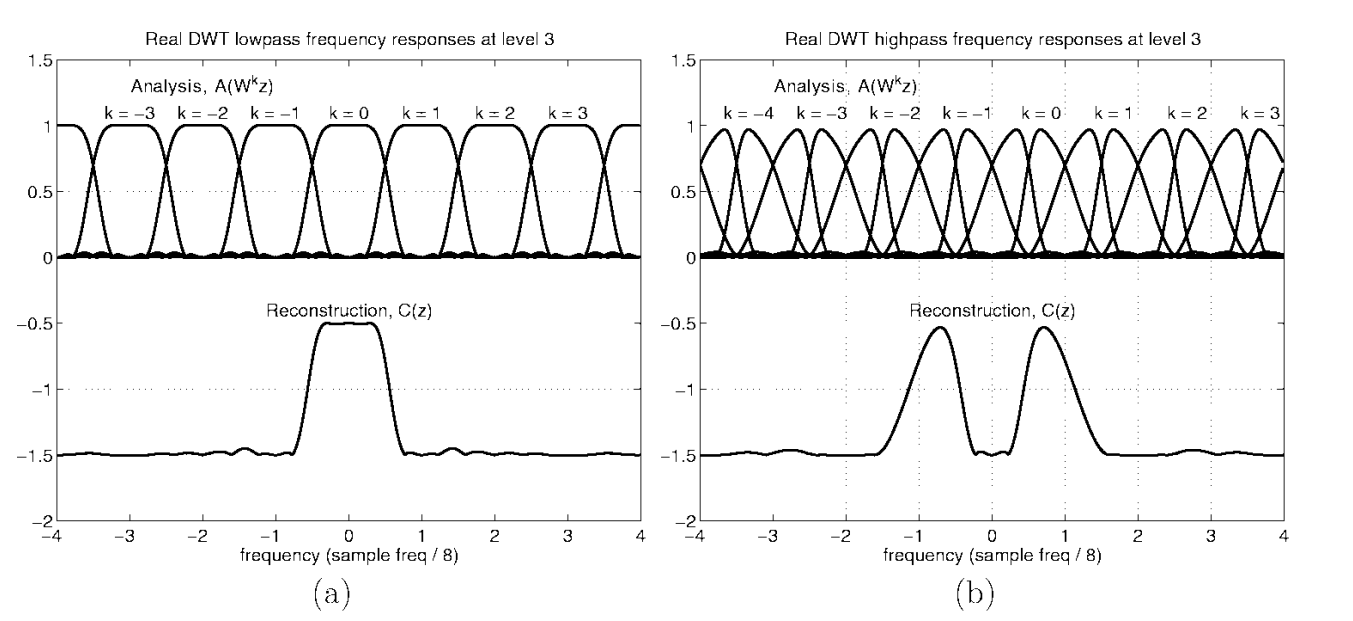
\includegraphics[width=\textwidth]{\imgpath/overlaps.png}
\end{figure}
To do this, let us consider the lowpass filters first. If we let:
\begin{align}
  B(z) &= z^{\pm M/2}A(z) \\
  D(z) &= z^{\mp M/2}C(z)
\end{align}
Then
\begin{align}
  A(W^kz)C(z) + B(W^kz)D(z) &= A(W^kz)C(z) + (W^kz)^{\pm M/2}A(W^kz) z^{\mp M/2}C(z) \\
  =& A(W^kz)C(z) + e^{\frac{jk2\pi}{M} \times (\pm \frac{M}{2})} z^{\pm M/2} z^{\mp M/2} A(W^kz)C(z) \\
  =& A(W^kz)C(z) + (-1)^k A(W^kz)C(z)
\end{align}
which cancel when k is odd.

Now consider the bandpass case. For shifts of $k=1$ the right half of the left
peak overlaps with the left half of the right peak. For a shift of $k=2$, the
left half of the left peak overlaps with the right half of the right peak.
Similarly for $k=-1$ and $k=-2$. For $|k| > 2$, there is no overlap. The fact
that we have overlaps at both even and odd shifts of $k$ means that we can't use
the same clever trick from before. However, what we do note is that the overlap
is always caused by opposite peaks (i.e. the left with the right peak, and never
the left with itself, or the right with itself). The solution then is to have
$B$ and $D$ have upper and lower passbands of opposite polarity, whil $A$ and
$C$ should have passbands of the same polarity.

Consider two prototype complex filters $P(z)$ and $Q(z)$ each with single
passbands going from $f_s/2M \rightarrow f_s/M$ (or $\frac{\pi}{M} \rightarrow
\frac{2*\pi}{M}$) - they must be complex to have support in only one half of the
frequency plane. Now say $P^*(z) = \sum_{r}p_r^*z^{-r}$ is the z-transform of
the conjugate of $p_r$, which has support only in the negative half of the
frequency plane. Then we can get the required filters by:
\begin{align}
A(z) &= 2\Re [P(z)] = P(z) + P^*(z) \\
B(z) &= 2\Im [P(z)] = -j[P(z) - P^*(z)] \\
C(z) &= 2\Re [Q(z)] = Q(z) + Q^*(z) \\
D(z) &= -2\Im [Q(z)] = j[Q(z) - Q^*(z)]
\end{align}
Then:
\begin{align}
  A(W^kz)C(z) + B(W^kz)D(z) = &  \left[P(W^kz) + P^*(W^kz)\right]\left[Q(z) + Q^*(z)\right] + \nonumber \\
                            & (-j*j)\left[P(W^kz) - P^*(W^kz)\right]\left[Q(z) - Q^*(z)\right] \\
                          = & P(W^kz)Q(z)[1+1] + P^*(W^kz)Q(z)[1-1] + \nonumber \\ 
                            & P(W^kz)Q^*(z)[1-1] + P^*(W^kz)Q^*(z)[1+1] \\
                          = & 2P(W^kz)Q(z) + 2P^*(W^kz)Q^*(z)
\end{align}

So now we only need to ensure that $P(W^kz)$ overlaps as little as possible with
$Q(z)$. This is somewhat more manageable, the diagram below shows the problem.

\begin{figure}
  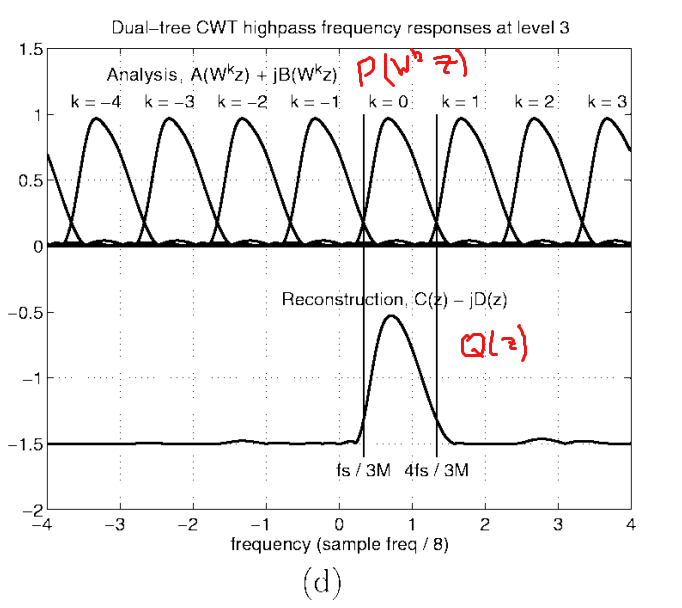
\includegraphics[width=\textwidth]{\imgpath/overlaps_complex.png}
\end{figure}

